\documentclass[ngerman,abstract=true]{scrartcl}
\usepackage{babel}
\usepackage{csquotes}

% typography
\usepackage{fontspec}
\setmainfont{Open Sans}[
  BoldFont={Open Sans Bold},
  ItalicFont={Open Sans Italic}]
\setsansfont{Open Sans}[
  BoldFont={Open Sans Bold},
  ItalicFont={Open Sans Italic}]
\setmonofont{Menlo}
\usepackage[factor=2000]{microtype}

% graphics, drawings, etc.
\usepackage{xcolor}
\usepackage{graphicx}
\usepackage[most]{tcolorbox}
\usepackage{tikz}
\usetikzlibrary{shapes.geometric}
\usetikzlibrary{shapes.arrows}
\usetikzlibrary{positioning}
\usetikzlibrary{matrix}
\newtcolorbox{anmerkung}{%
  grow to left by=10pt,
  colback=black!10,
  colframe=white,
  coltitle=black,
  borderline west={4pt}{0pt}{black!30},
  boxrule=0pt,
  boxsep=0pt,
  %breakable,
  enhanced jigsaw,
  title={Anmerkung\par},
  fonttitle={\bfseries},
  attach title to upper={}}

% highlighting, lists, code
\usepackage{soul}
\usepackage{enumitem}
\usepackage{listings}
\lstset{
  basicstyle=\ttfamily,
  escapeinside=||,
  keywordstyle=\color{blue!50!black},
  stringstyle=\color{green!50!black}}

% nice tables
\usepackage{booktabs,array}
\newcommand{\tablespacing}[1]{\renewcommand{\arraystretch}{#1}}

% links
\usepackage[
  colorlinks,
  linkcolor={red!50!black},
  citecolor={blue!50!black},
  urlcolor={blue!80!black}
]{hyperref}

\title{Betriebssysteme}
\date{Wintersemester 2018-2019}
\author{Prof.\ Neeraj Suri, Dr.\ Stefan Winter}

\begin{document}
\maketitle
  
\tableofcontents
\newpage
  
\section{Geschichte}

Am Anfang gab es noch keine Betriebssysteme, alle Programme liefen direkt auf der Hardware (\emph{Bare Metal}). Da jedes Programm in irgendeiner Weise Daten verarbeiten muss, musste man für jedes Programm gewisse Eingaben zugänglich machen, und gewisse Ausgaben in einer für dem Benutzer nutzbaren Art ausgeben. Also musste man Code schreiben, der eigentlich garnichts mit dem Programm zu tun hat, sondern nur dazu dient, diese Eingaben und Ausgaben zu ermöglichen.

\begin{figure}[h]\centering
\begin{tikzpicture}[
  code/.style={rectangle, draw, rounded corners, text width=5.5cm, align=left}]
\node[code,label={\textbf{Code}}] (code) {\verb|get_user_input();|\\\verb|do_processing();|\\\verb|generate_user_output();|};
\node[label=below:{\textbf{Output}}] (screen) at (-4,-3) {
\includegraphics[width=3cm]{media/screen}};
\node[label=below:{\textbf{Input}}] (input) at (0,-3) {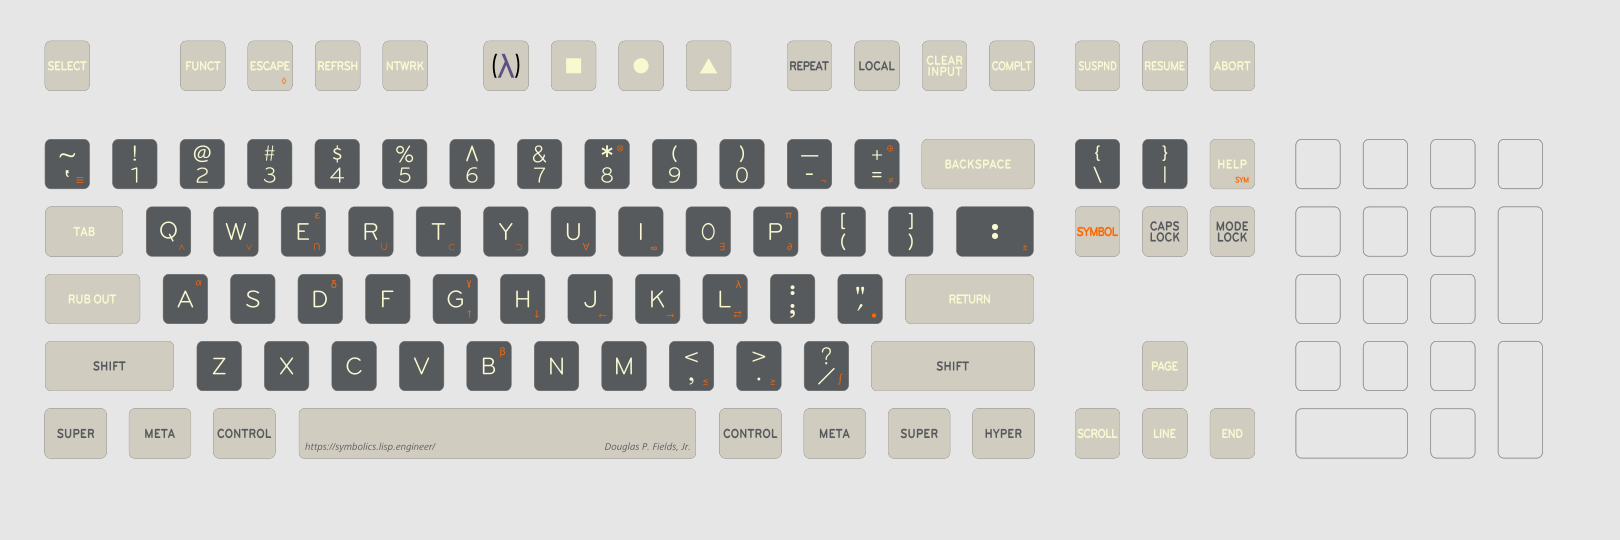
\includegraphics[width=4cm]{media/keyboard}};
\node[label=below:{\textbf{Storage}}] (storage) at (4,-3) {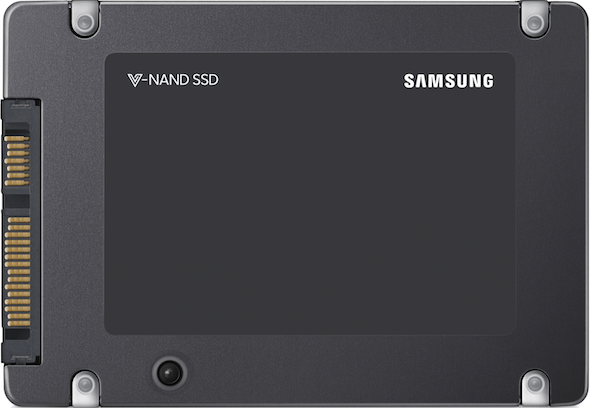
\includegraphics[width=3cm]{media/ssd}};
\draw[<->] (code) -- ++(-4,0) -- (screen);
\draw[->] (code) -- (input);
\draw[->] (code) -- ++(4,0) -- (storage);
\end{tikzpicture}
\caption{Programmierung auf Hardware ohne Abstraktion}\label{fig:prog}
\end{figure}

\subsection{Library}

Irgendwann erkannte man dann, dass man sehr oft gewisse Funktionalität neu implementieren musste, weil unterschiedliche Programme ähnliche Eingaben erwarteten oder ähnliche Ausgaben erzeugten, und man diesen Code dafür widerholte. Eine Idee hier ist, den Code, den man häufig verwendet, in eine \emph{Library} packt. Damit können diese Routinen wiederverdendet werden. Außerdem können Programme sich so mehr auf ihre eigentlichen Aufgaben konzentrieren.

\begin{figure}[h]\centering
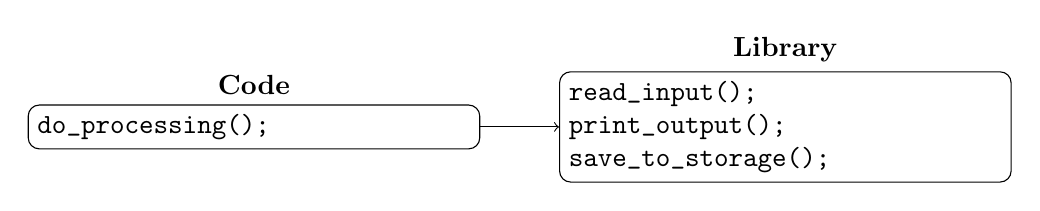
\begin{tikzpicture}[
  code/.style={rectangle, draw, rounded corners, text width=5.5cm, align=left}]
\node[code,label={\textbf{Code}}] (code) {\verb|do_processing();|};
\node[code,label={\textbf{Library}},right=of code] (library) {\verb|read_input();|\\\verb|print_output();|\\\verb|save_to_storage();|};
\draw[->] (code) -- (library);
\end{tikzpicture}
\caption{Ausbau von Funktionen in eine Library}\label{fig:library}
\end{figure}

Der Nachteil von diesem Ansatz war, dass diese Libraries immer wieder umgeschrieben mussten, wenn ein anderer Computer verwendet wurde.

\subsection{Exponentielles Wachstum von Hardwarekomplexität}

\begin{figure}\centering
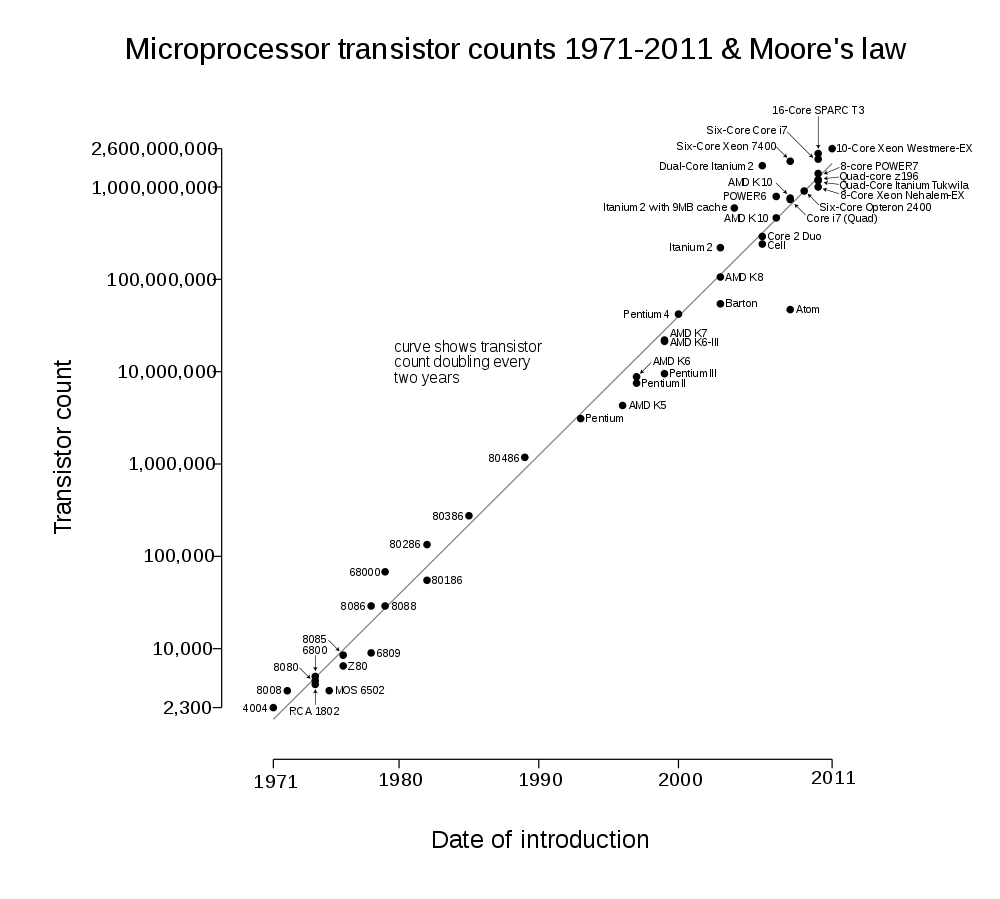
\includegraphics[trim={1.8cm 1.8cm 1cm 3.6cm},clip,width=0.8\linewidth]{media/mooreslaw}
\caption{Hardwarekomplexitätswachstum seit 1971.}\label{fig:mooreslaw}
\end{figure}

Es ergab sich also die Schwierigkeit, dass die Hardware sich so rasant entwickelt. Dies ist in Abbildung \ref{fig:mooreslaw} graphisch aufgezeigt, wobei man anmerken muss, dass die Skala logarithmisch ist. Das scheinbar lineare Wachstum der Transistoranzahl ist also tatsächlich ein exponentielles. Das nennt man auch Moore's law, nach dem Begründer von Intel.

\subsection{Heute}

\begin{figure}[p]\centering
\begin{tikzpicture}
\node (phone) {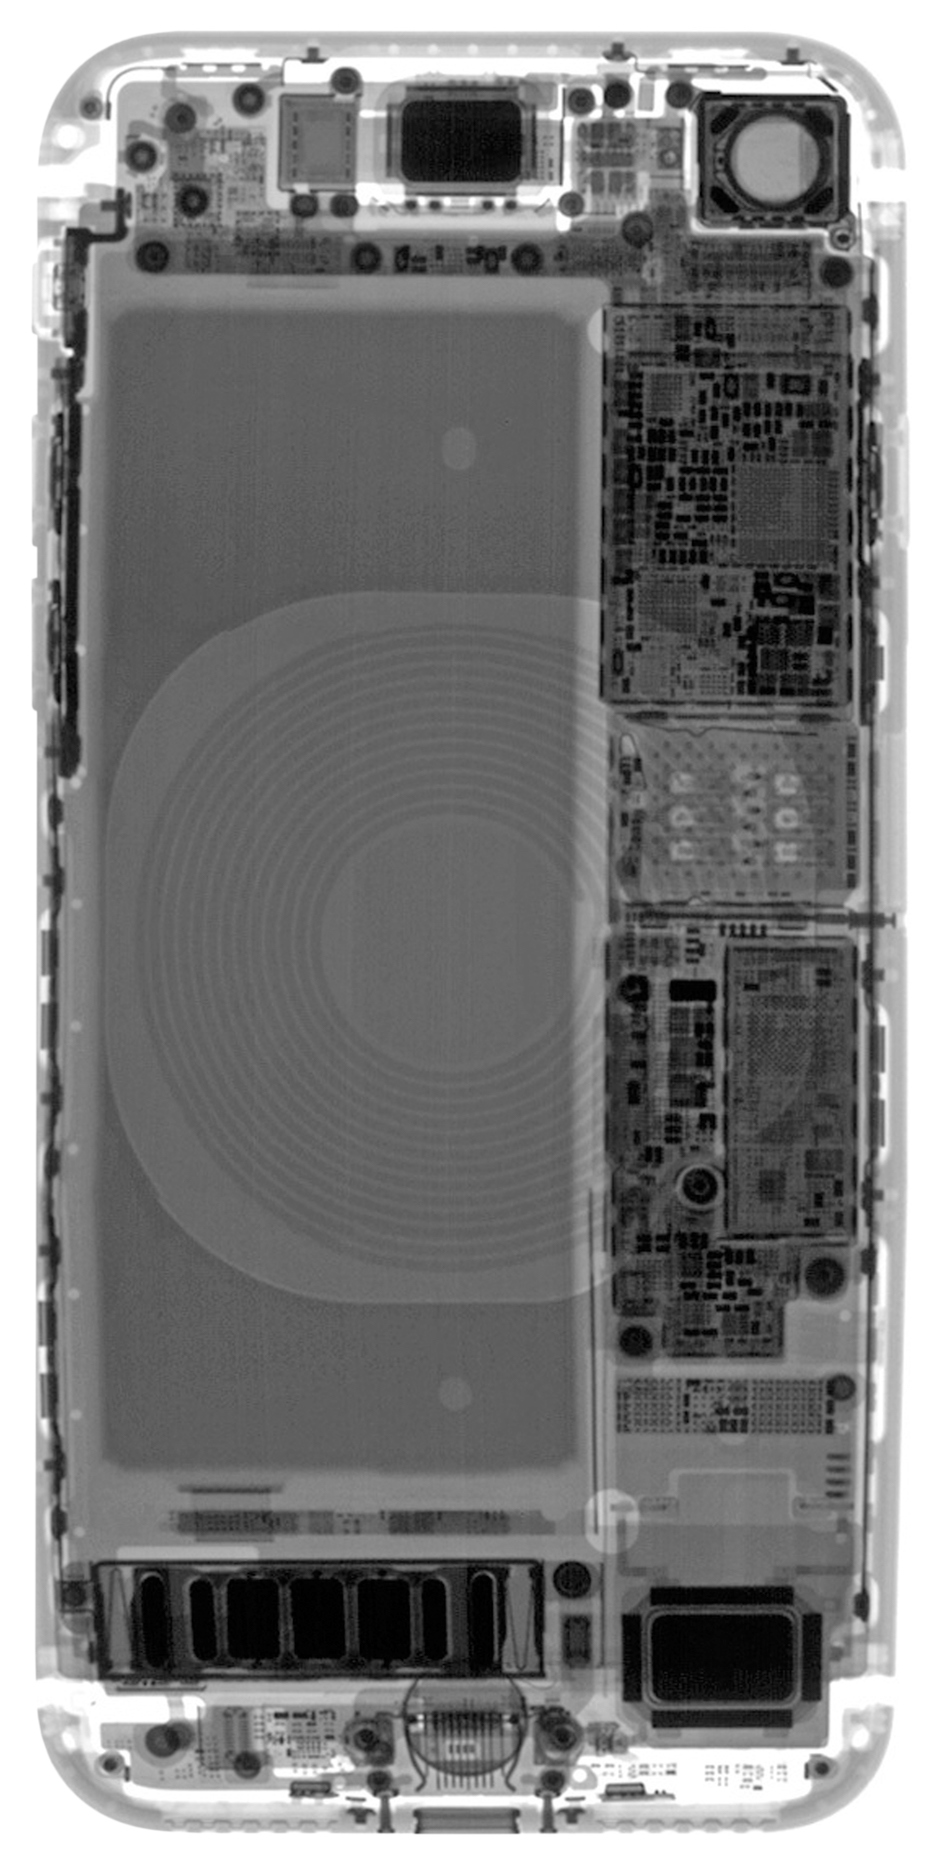
\includegraphics[width=8cm]{media/phone}};
\draw[very thick, white] (1.3,3.1) rectangle (3.2,4.9) node[pos=.5] {\textbf{A11}};
\draw[very thick, white] (1.3,2.1) rectangle +(1,0.9) node[pos=.5] {\textbf{QM}};
\draw[very thick, white] (2.1,-0.8) rectangle +(1.1,0.8) node[pos=.5] {\textbf{SW}};
\node[text width=6cm,align=left] (a11) at (7,6) {\textbf{Apple A11 SoC}\\Betriebssystem: iOS (Darwin), UNIX-Derivat, POSIX kompatibel.};
\node[below=5mm of a11, text width=6cm,align=left] (se) {\textbf{Apple Secure Enclave}\\Im A11-Chip eingebaut\\Betriebssystem: Basiert auf dem L4 Mikrokernel};
\node[below=5mm of se, text width=6cm,align=left] (qc) {\textbf{Qualcomm Snapdragon X16}\\LTE Modem\\Betriebssystem: Unbekanntes RTOS, eventuell REX OS};
\node[below=5mm of qc, text width=6cm,align=left] (skyone) {\textbf{Skyworks SkyOne SKY78140}\\CDMA Modem\\Betriebssystem: Unbekannt};
\end{tikzpicture}
\caption{Betriebssyteme auf Konsumergeräten am Beispiel iPhone}\label{fig:osdevices}
\end{figure}
\begin{figure}[p]\centering
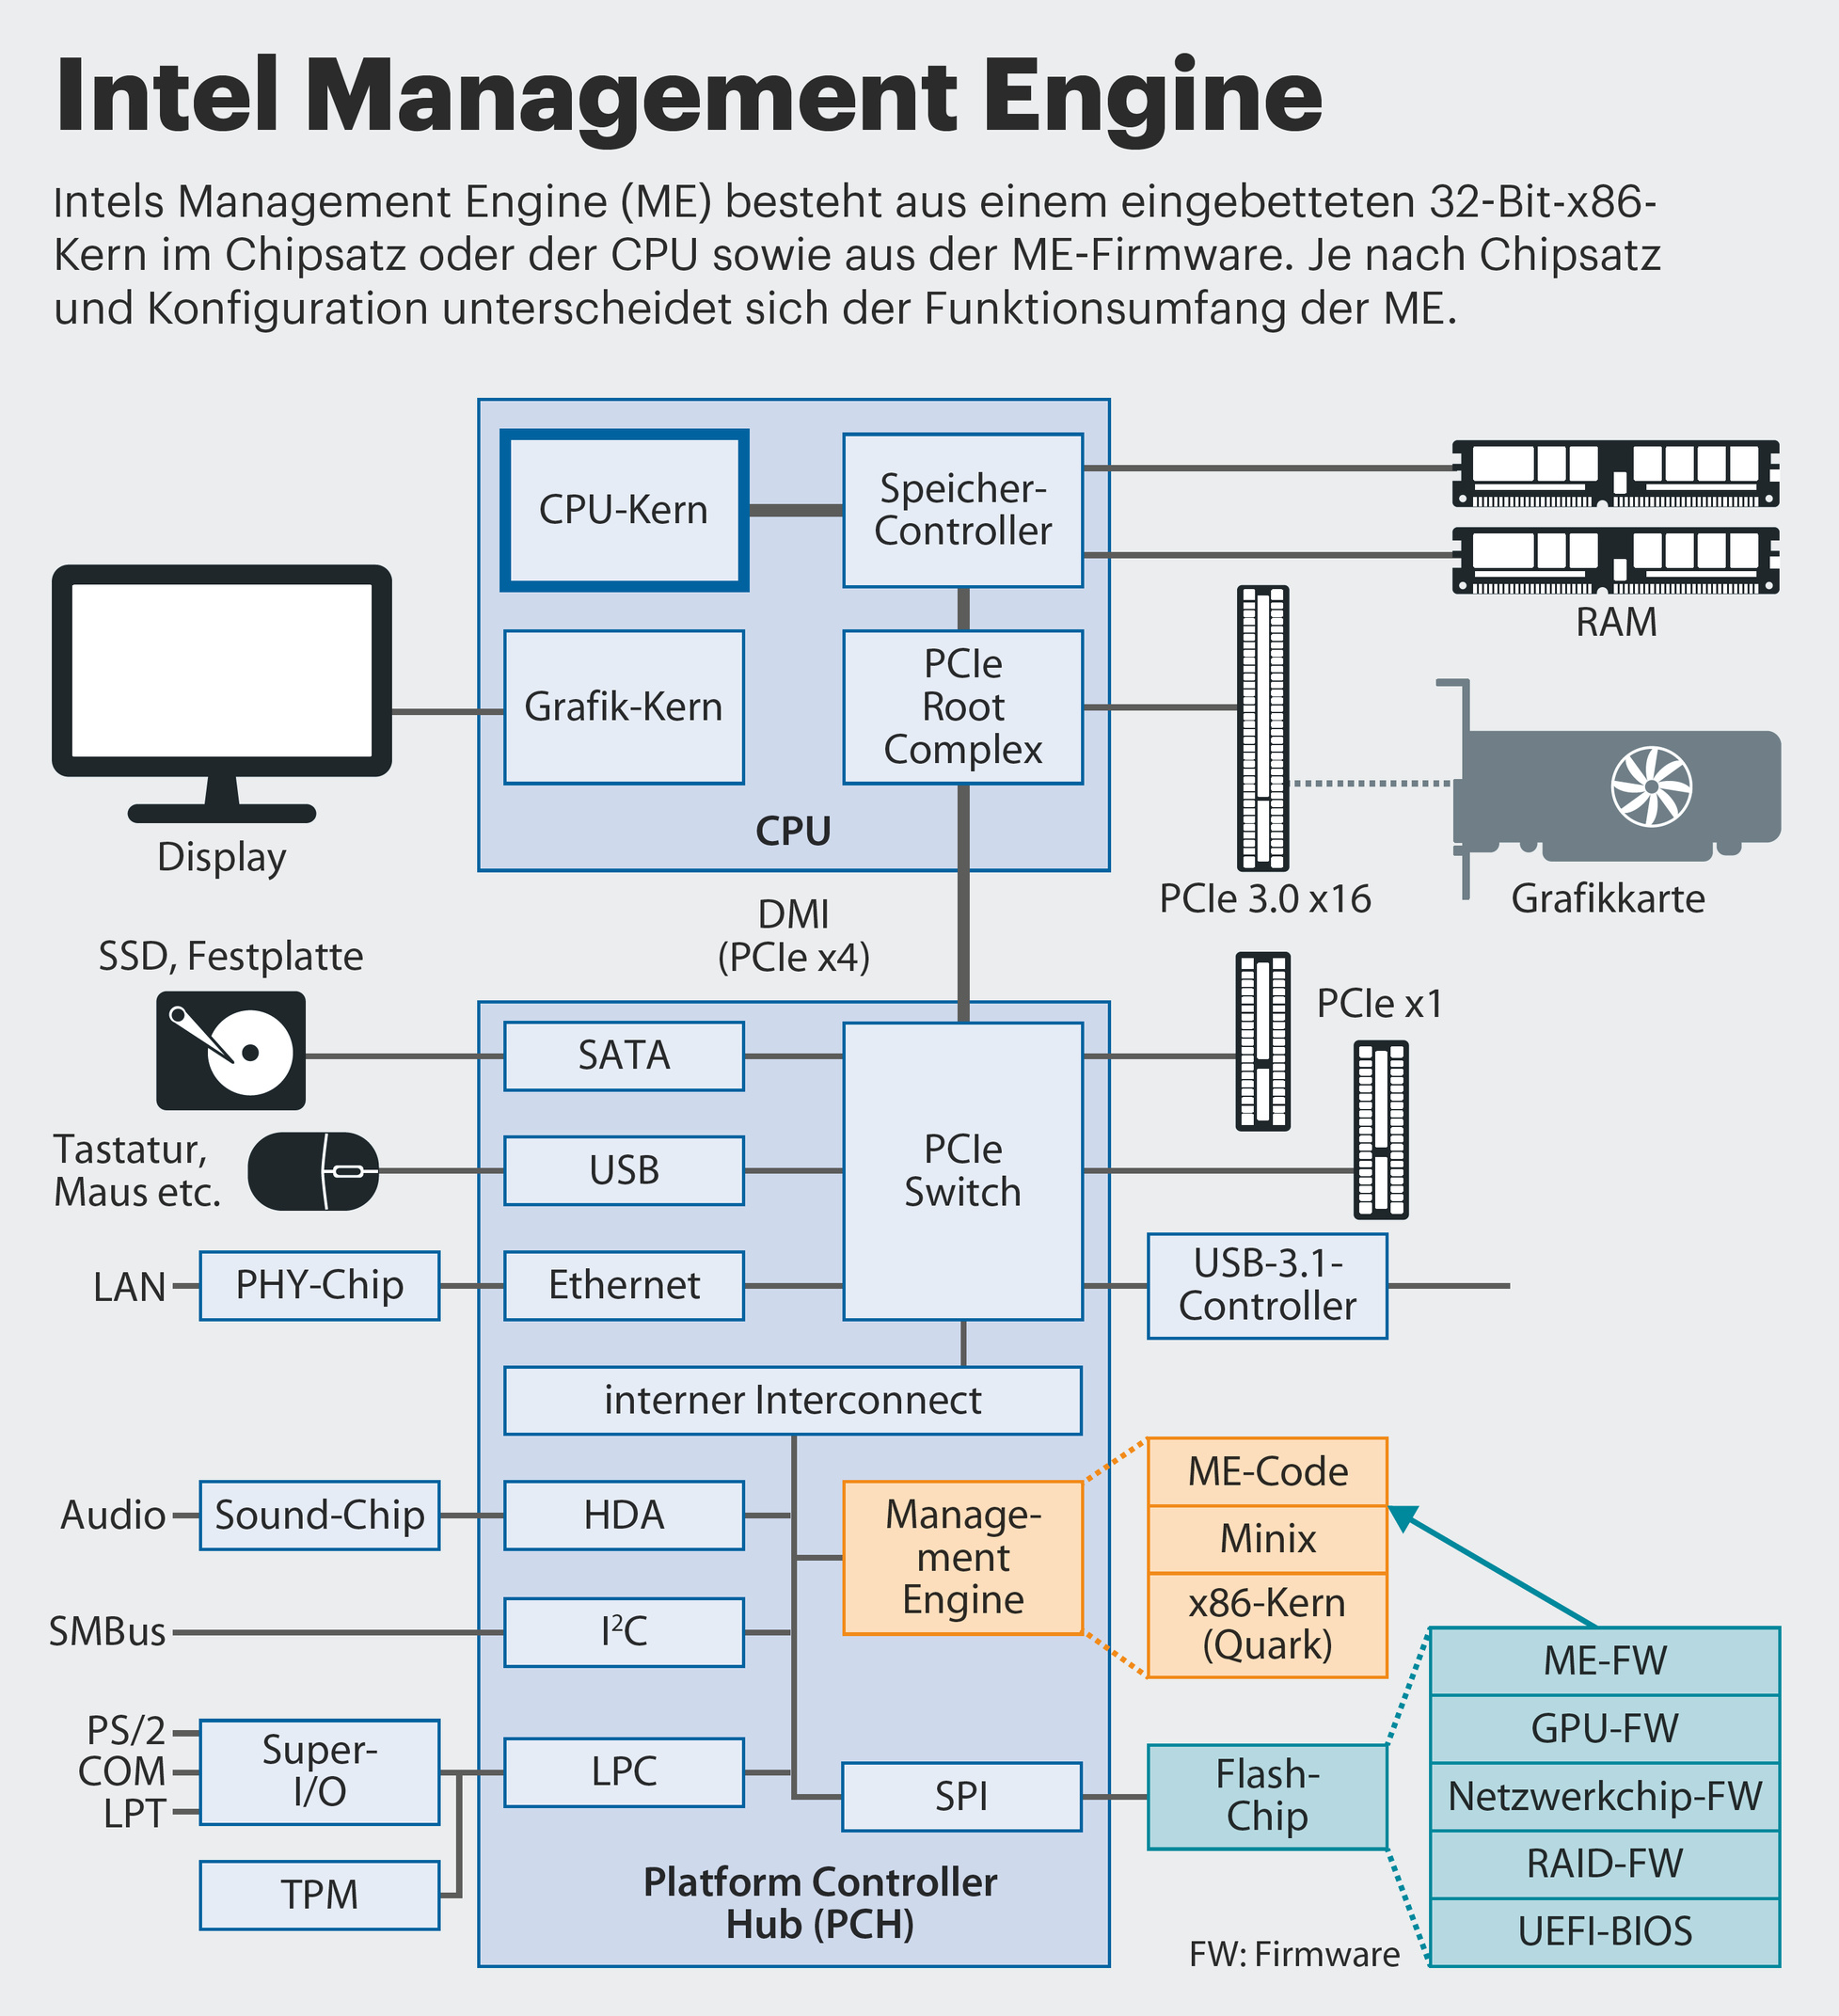
\includegraphics[width=0.8\textwidth]{media/intelme}
\caption{Intel Management Engine. Quelle: Heise.de}\label{fig:intelme}
\end{figure}

Heutzutage sind Betriebssysteme \emph{überall}. Von Fernsehehern zu Autos, Servern, Handys bis hin zu Operationssälen. Interessanterweise sind teilweise mehrere Betriebssysteme auf einem Gerät zu finden. Abbildungen \ref{fig:osdevices} und \ref{fig:intelme} zeigen, dass sogar in den Geräten, die wir tagtäglich verwenden, oft mehr steckt, als wir denken.

Die Betriebssysteme, die wir benutzen, haben oft sehr viele Features eingebaut. 

\section{Definition}

Wie definiert man eigentlich, was ein Betriebssystem ist, und was nicht? Dazu gibt es nicht nur eine, sondern gleich mehrere Definitionen. 

\subsection{Hardwareabstraktion}

Man kann ein Betriebssystem als eine Hardwareabstraktionsschicht beschreiben. Das Betriebssytem ist als dafür zuständig, eine Ausführungsumgebung zu erstellen für die Programme, die darauf laufen sollen. Dazu muss das Betriebssystem den Programmen eine Abstraktionsebene bieten, damit diese nicht direkt mit der Hardware interagieren müssen. Außerdem muss das Betriebssyste die Resourcen verwalten und (idealerweise fair) zwischen den Programmen teilen.

Wenn man sich jetzt mal anschaut, wie viel Code eigentlich hinter der Ausführung eines kleinen, simplen Programms steckt, dann merkt man, wie viel eigentlich hinter den Kulissen passieren muss, damit die Programme das tun, was wir von ihnen erwarten. In Abbildung \ref{fig:hardwareabstraktion} ist zu sehen, welche Ebenen eigentlich unter einen Programm liegen, und wie viel Code diese Beinhalten.
\begin{figure}[!h]\centering\tablespacing{1.4}
\begin{tabular}{@{}p{3.4cm}p{2.6cm}r@{}}
\toprule
\textbf{Ebene} & \textbf{Beispiel} & \textbf{Zeilen}\\
\midrule
Java Bytecode 
  & & \textasciitilde 1\,000\\
Java Runtime 
  & \verb|openjdk11| & 8\,047\,913\\
Support Libraries 
  & \verb|glib| & 460\,641\\
  & \verb|libcxx| & 441\,343\\
System Libraries 
  & \verb|glibc| & 1\,384\,092\\
Kernel 
  & \verb|darwin| & 1\,070\,917\\
  & \verb|openbsd| & 2\,235\,267\\
  & \verb|netbsd| & 5\,930\,334\\
  & \verb|linux| & 17\,120\,205\\
  & \verb|windows| & \textasciitilde 65\,000\,000\\
Hardware &&\\
\bottomrule 
\end{tabular}
\caption{Hardwareabstraktionsebenen und Codegröße}\label{fig:hardwareabstraktion}
\end{figure}

\begin{anmerkung}
Ich habe mir mal die Freiheit genommen, die Zeilen Sourcecode für die meisten Projekte hier durchzuzählen. Dazu habe ich das Programm \verb|cloc| benutzt (auf macOS mit \verb|brew install cloc| installierbar). Die \verb|libcxx| ist die C++ Standard Library, die vom Clang Compiler des LLVM Projekt genutzt wird (wird verwendet von iOS, macOS, Linux, usw.). Der macOS Kernel, \verb|darwin|, ist Quelloffen, deswegen habe ich den auch mitgenommen. Allerdings muss man dazu sagen, dass dieser modular aufgebaut ist, und hier keine Module mitgenommen wurden, deswegen sind die Resultate nicht direkt verlgeichbar. Bei den BSD Kerneln habe ich nur den \verb|sys/|-Ordner ausgewertet, da die anderen Ordner nicht unbedingt zum Kernel gehören (sondern Libraries, Compiler, usw. sind). Außerdem beinhalten die Angaben von Windows mehr als nur den Kernel, auch diese Angaben sind also nicht vergleichbar. 
\end{anmerkung}


Außerdem musste man ja.

\subsection{Kernel und Systemlibraries}

Man könnte ein Betriebssystem so definieren, indem man sagt, dass es die Summe aus Kernel und Systemlibraries ist. Dazu müsste man aber definieren, was Systemlibraries sind. Dazu gibt es netterweise einige Standards. Die wichtigsten und interessantesten sind POSIX, was für \emph{Portable Operating System Interface} steht, und LSB, was für \emph{Linux Standard Base} steht.

Diese Standards existieren, weil man eine Kompatibilität zwischen verschiedenen Betriebssystemen herstellen möchte. Das bedeutet, dass man sein Programm einmal schreiben kann, und es theoretisch auf unterschiedlichen Betriebssystemen laufen lassen kann. 
\begin{table}[h]\centering\tablespacing{1.3}
\begin{tabular}{@{}lp{10cm}@{}}
\toprule
\textbf{Standard} & \textbf{Betriebssysteme}\\
\midrule
POSIX 
  & macOS (Zertifiziert seit 10.5 Leopard)\\
  & Solaris\\
  & Android\\
  & Windows (nicht Out-of-the-Box, aber mit Cygwin, MinGW oder neuerdings dem \emph{Windows Subsystem for Linux})\\
LSB
  & Debian (teilweise)\\
\bottomrule
\end{tabular}
\caption{Betriebssystemstandards}\label{tbl:osstd}
\end{table}
In Tabelle \ref{tbl:osstd} sieht man eine Liste von Betriebssystemstandards, und die Betriebssysteme, die zumindest halbwegs konform sind. Wie man sehen kann, können und werden auch teilweise sehr wilde Architekturen (Windows) konform gemacht, weil dadurch viele Vorteile entstehen können, in diesem Fall Zugriff auf Open-Source Libraries und Tools, die auf Linux oder macOS laufen.

\subsection{Kernel-Mode}

Wenn man schon Kernel und Systemlibraries zusammen ein \emph{Betriebssysten} nennt, was ist denn dann bitte ein Kernel? Typischerwise würde man sagen, dass man als Kernel all das bezeichnet, was auf dem Prozessor im \emph{Kernel-Mode} läuft.

Viele Prozessoren, unter anderem x86-CPUs, haben ein \enquote{Ring}-System, mit dem der Zugriff auf privilegierte Instruktionen limitiert wird. Der Kernel läuft bei einem solchen System im Ring 0 (der Kernel-Mode), während reguläre Programme im Ring 3 laufen (dem User-Mode). 

\begin{figure}[h]\centering
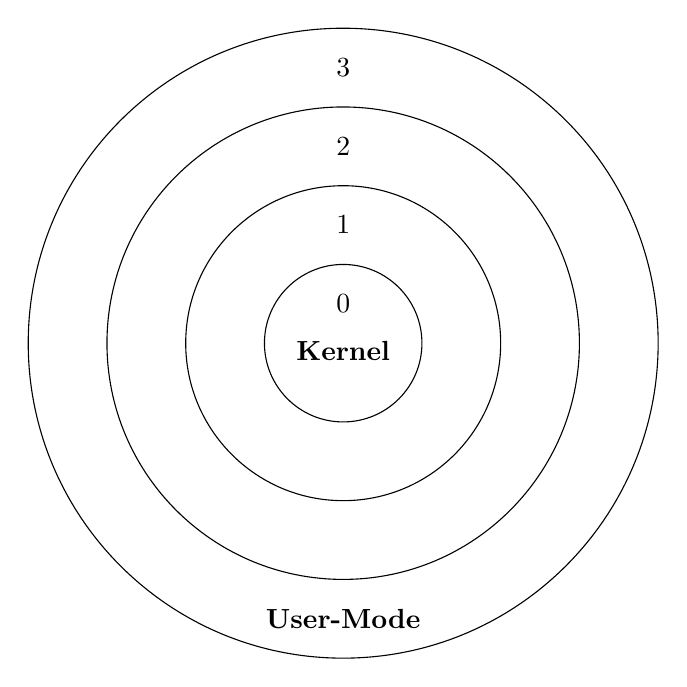
\begin{tikzpicture}
  \draw circle[radius=4cm] node[yshift=3.5cm] {3} node[yshift=-3.5cm] {\textbf{User-Mode}};
  \draw circle[radius=3cm] node[yshift=2.5cm] {2};
  \draw circle[radius=2cm] node[yshift=1.5cm] {1};
  \draw circle[radius=1cm] node[yshift=.5cm] {0} node[yshift=-0.1cm] {\textbf{Kernel}};
\end{tikzpicture}
\caption{Das Ring-System bei x86 Prozessoren.}\label{fig:ringsystem}
\end{figure}
Reguläre Anwendungen haben somit also keinen direkten Zugriff auf die meisten Systemresourcen. Programme können nicht direkt auf die Festplatte zugreifen, sondern müssen den Kernel nett darum bitten, dies doch bitte für sie zu tun.

Diese Definition ist leider nicht immer nützlich, denn auf manchen Systemen gibt es diesen Unterschied zwischen privilegiertem und regulärem Code nicht. Aber das wirft auch eine andere Frage auf, was für Funktionalität packen wir eigentlich in den Kernel, und was nicht?

\subsection{Monolithische- und  Mikrokernel}

Es gibt zwei Arten von Kerneln, die man Unterscheiden kann; diese sind \emph{Monolithische-} und \emph{Mikrokernel}. Der hauptsächliche Unterschied unter den beiden ist wie viel Code im Kernel-Mode läuft. 
\begin{figure}[tbp]\centering
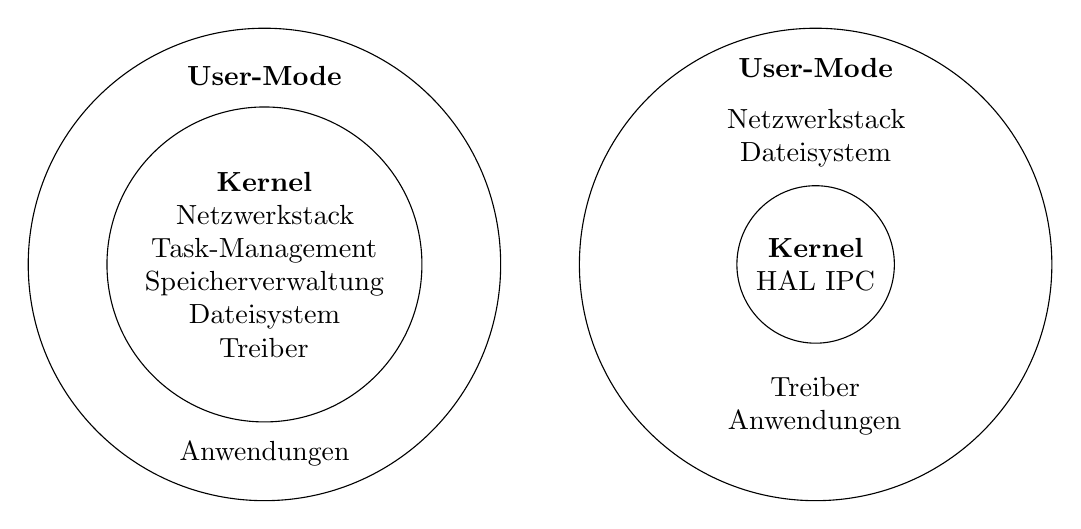
\begin{tikzpicture}
  \draw circle[radius=3cm] circle[radius=2cm] node[text width=3.5cm,text centered] {\textbf{Kernel}\\Netzwerkstack\\Task-Management\\Speicherverwaltung\\Dateisystem\\Treiber} node[yshift=2.4cm] {\textbf{User-Mode}} node[yshift=-2.4cm] {Anwendungen};
  \draw (7,0) circle[radius=1cm] circle[radius=3cm] node[text width=2cm,text centered] {\textbf{Kernel}\\HAL IPC} node[yshift=2.5cm] {\textbf{User-Mode}} node[yshift=1.6cm,text width=4cm,text centered] {Netzwerkstack\\Dateisystem} node[yshift=-1.8cm,text width=4cm,text centered] {Treiber\\Anwendungen};
\end{tikzpicture}
\caption{Übersicht über die Architektur Monolithischer- und Mikrokernel.}\label{fig:monolith}
\end{figure}
Abbildung \ref{fig:monolith} zeigt, wie die Architektur in etwa aufgebaut ist bei den verschiedenen Typen von Kerneln.

Es gibt unterschiedliche Gründe, Monolithische oder Mikrokernel zu verwenden. Die meisten Kernel, die in Endnutzersystemen benutzt werden (macOS, Linux, Windows), sind Mikrokernel. Das liegt einfach daran, dass Mikrokernel generell schneller sind.
\begin{figure}[p]
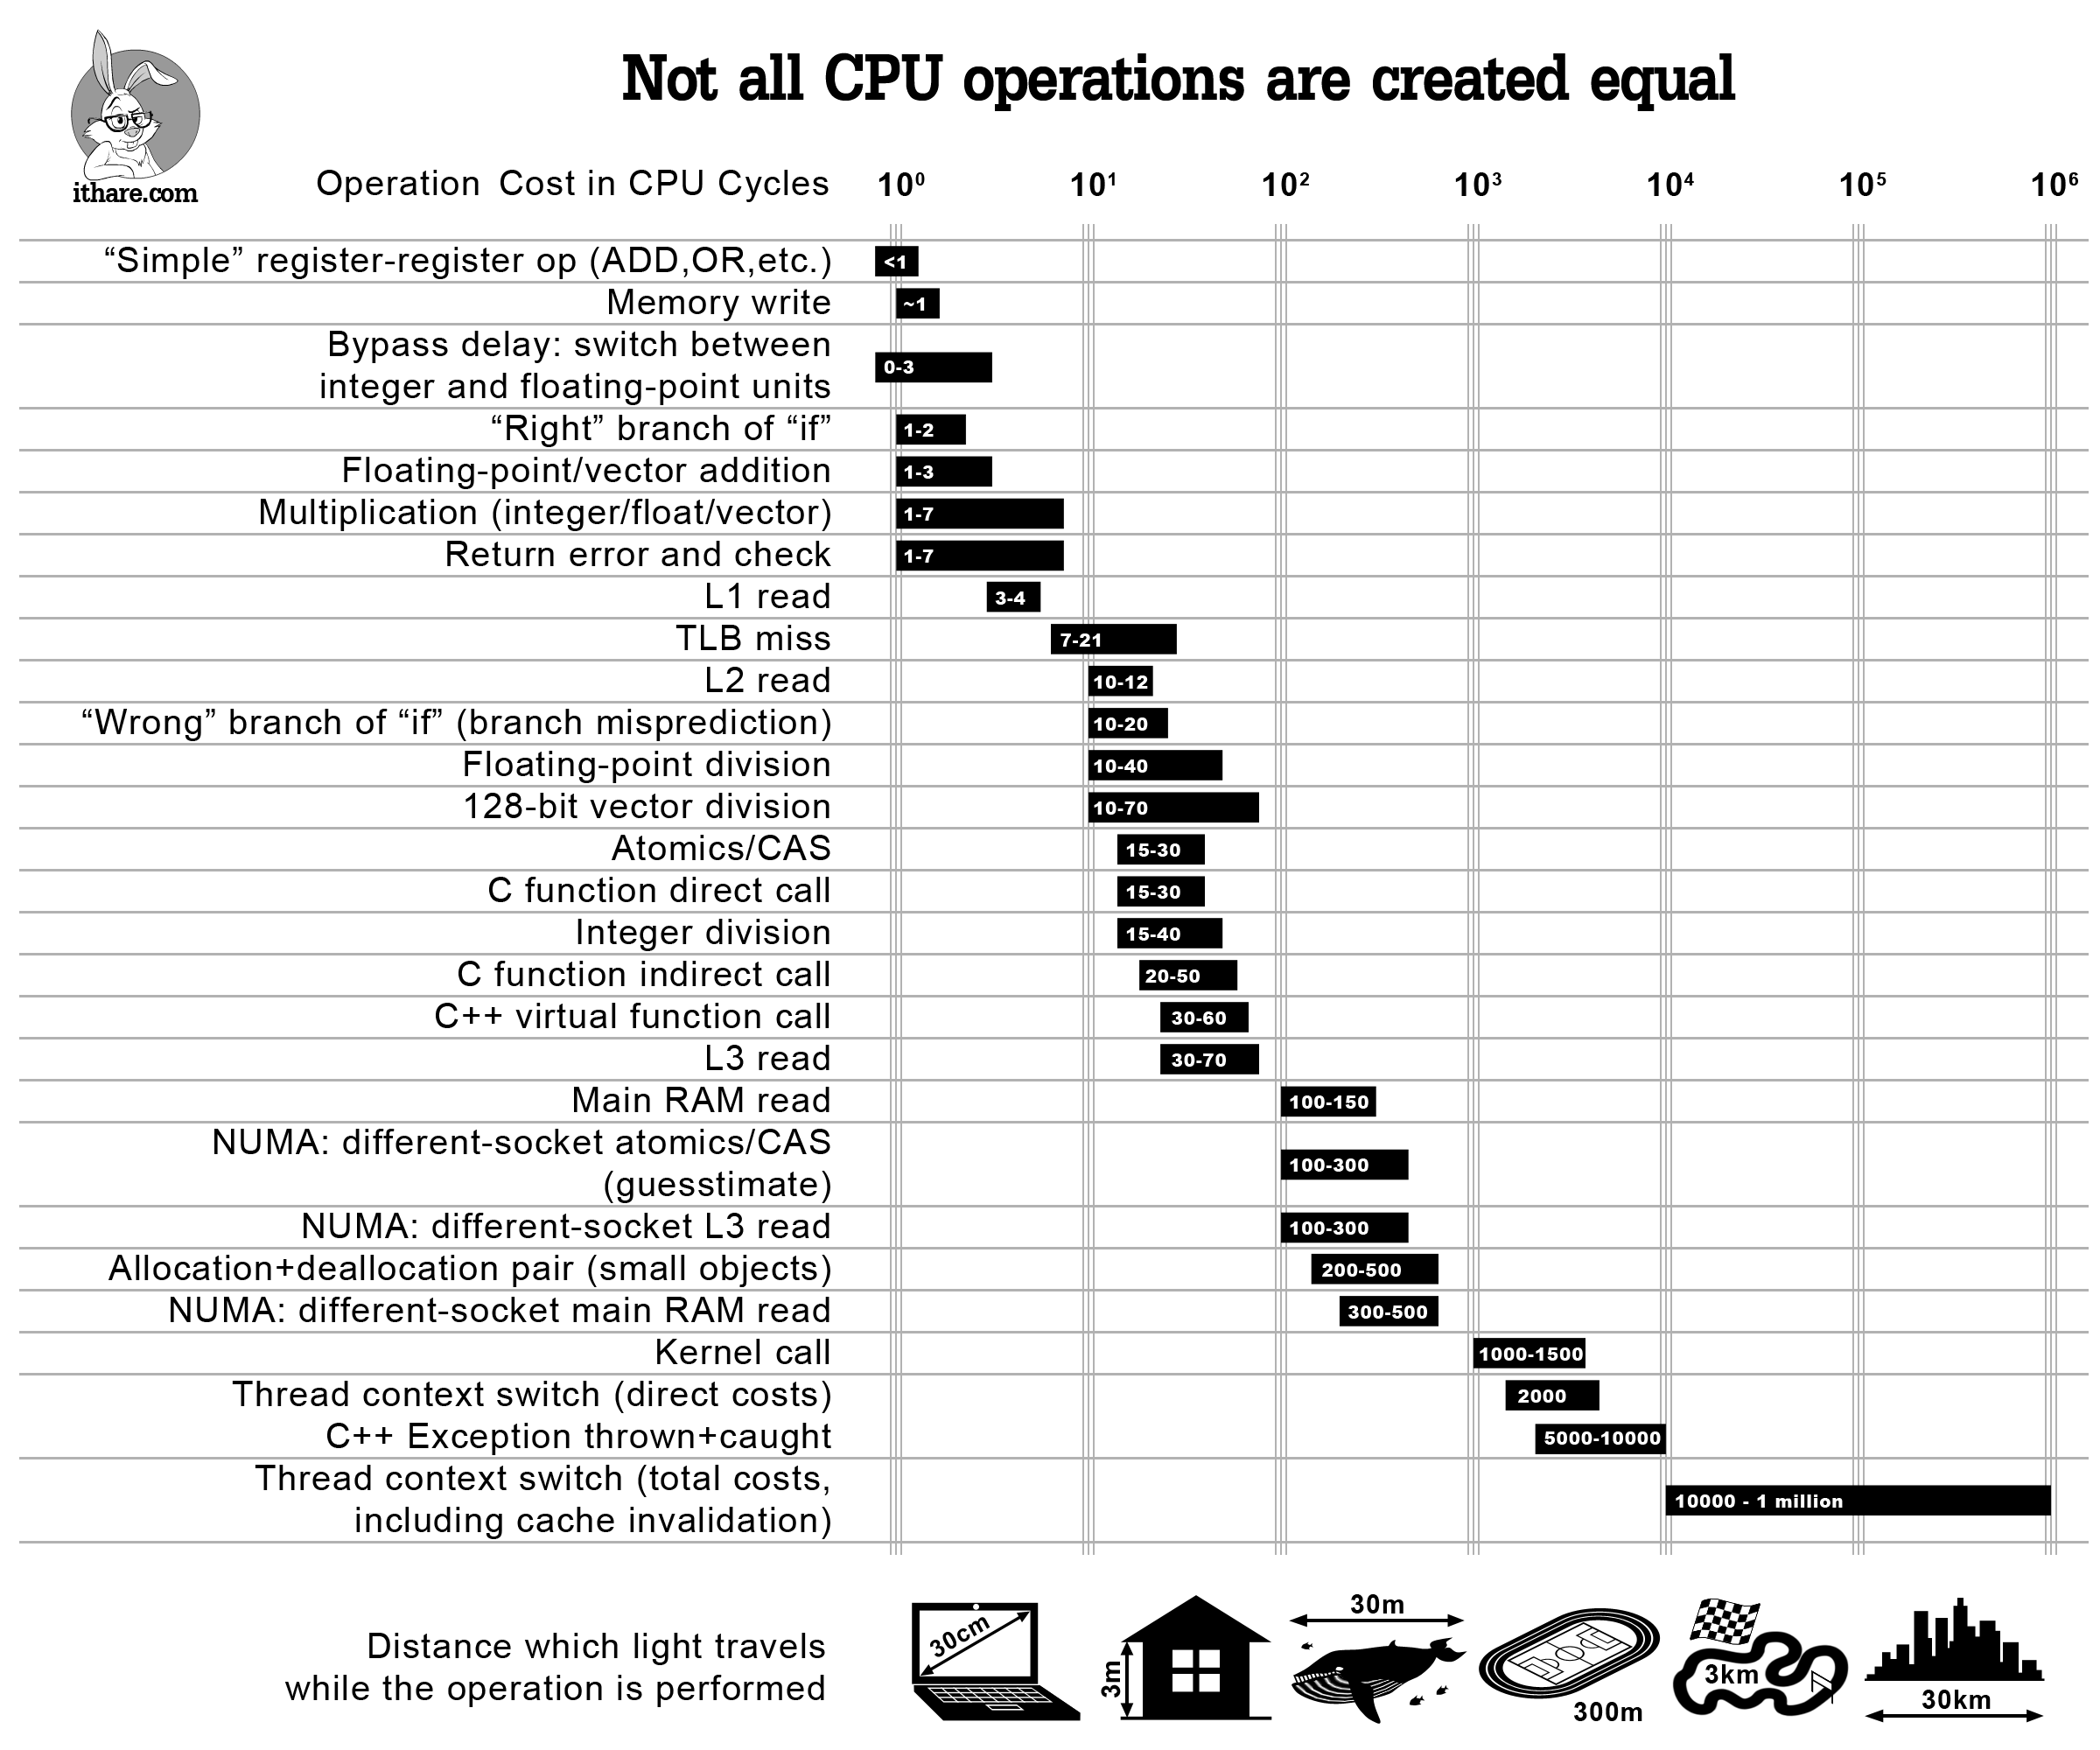
\includegraphics[width=\textwidth]{media/infographic}
\caption{Übersicht über die Kosten verschiedener Operationen.\newline Quelle: \url{http://ithare.com}.}\label{fig:infographic}  
\end{figure}
Abbildung \ref{fig:infographic} zeigt, wie viele CPU Zyklen gewisse Operationen brauchen. Dort sieht man, dass ein Kernelaufruf (also ein Switch vom User-Mode in den Kernel-Mode und wieder zurück) stolze 1000 bis 1500 CPU-Zyklen braucht. Warum ist das so? Wenn der CPU einen solchen Kontextswitch macht, müssen viele CPU-Internen Datenstrukturen zurückgesetzt werden, zum Beispiel den \emph{Translation Lookaside Buffer}, weil der Kernel eine andere Sicht auf den Speicher hat. Der Status des CPUs muss gespeichert werden (also alle Register, wenn der Kernel Gleitkommazahlberechnungen machen muss, dann müssen auch alle Floating-Point-Register gespeichert werden) damit der CPU nach dem Systemcall in den selben Zustand versetzt werden kann, wie er davor war. Außerdem müssen viele Caches weggeworfen werden. Da Switches zwischen Kernel- und User-Mode so teuer sind, versucht man, so viel wie möglich direkt im Kernel zu machen. 

Es gibt aber auch Nachteile bei einer solchen Architektur. \hl{Alles, was im Kernel läuft, ist ein potenzielles Sicherheitsproblem, denn es hat uneingeschränkt Zugriff auf alles}. Wenn ein Programm abstürzt, kann es dem System nicht schaden, weil alle Zugriffe auf Resources vom Kernel abgefangen werden. Wenn ein Treiber abstürzt, gibt es aber kein Sicherheitsnetz. Daher kommen Bluescreens (bei Windows) oder Kernel Panics (bei Linux).

Die Mikrokernelarchitektur hat einen anderen Ansatz. Hier versucht man, so \emph{wenig} wie möglich im Kernel-Mode laufen zu lassen. Man macht hier nur das absolut notwendige: man bietet eine Hardwareabstraktionsschicht und einen Mechanismus, mit dem Prozesse kommunizieren können. 

Die Idee dahinter ist, dass man Funktionalität, die sonst im Kernel wäre, einfach im Userspace laufen lässt. Treiber laufen dann als reguläre Prozesse, und Anwendungen können mit IPC Anfragen stellen. Die Vorteile hier sind Sicherheit und Stabilität, denn nur das Allernötigste läuft mit maximalen Rechten. Wie man vorhin gesehen hat, hat Apple in iPhones einen Subprozessor, die \emph{Secure Enclave}, die unter anderen Verschlüsselungskeys verwaltet. Diese nutzt einen Mikrokernel, genauso wie das Merkel-Phone und gewisse andere Sicherheitsrelevante Produkte.

\subsection{Koordination}

Ein Betriebssytem kann man auch Ressourcenverwaltung ansehen. Es verwaltet die Ressourcen, die einem System zur Verfügung stehen. Dazu gehören zum Beispiel Speicher, Rechenleistung und Peripheriegeräte. Das Betriebssystem sorgt dafür, dass jedes Programm die Ressourcen effizient und fair nutzen kann.

Das Betriebssystem kontrolliert die Ausführung von Programmen, um Fehler und falsche Verwendung von Ressourcen zu verhindern.


\end{document}










